\documentclass{article}
\usepackage{graphicx}
\graphicspath{ {./images/} }
\usepackage{amsmath}
\usepackage{gensymb}

\title{9. Kompleksie skaitļi - trigonometriskais pieraksts}
\author{Gunārs Ābeltiņš}
\date{2023-05-17}

\begin{document}

\maketitle

\section*{1. uzdevums}
Attēlojiet plaknē un atrodiet no attēla aptuvenus trigonometriskos pierakstus šādiem skaitļiem: 5, -5, 5i, -5i, -5+5i, 2+5i, 2-5i, -2+5i, -2-5i.

$$ a+bi = r(\cos \varphi + i\sin \varphi)$$

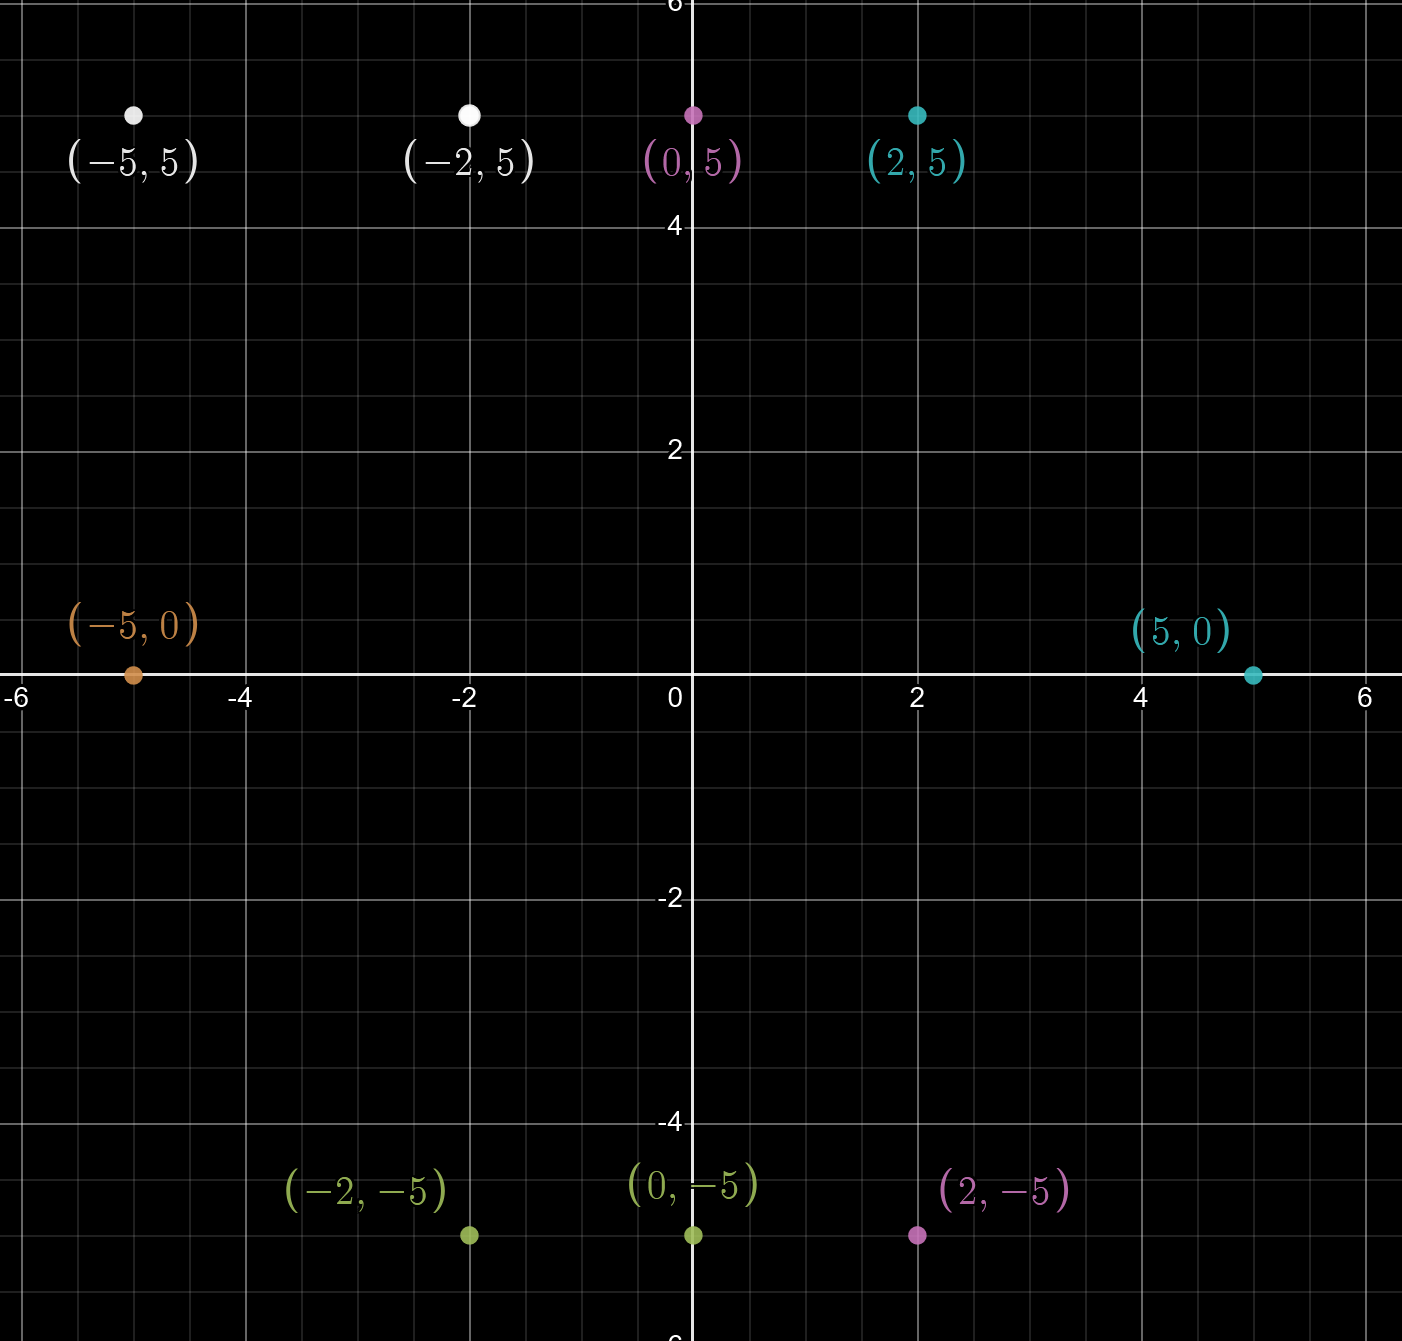
\includegraphics[width=\textwidth]{1}

$$ 5 = 5(\cos 0\degree + i\sin 0\degree)$$
$$ -5 = 5(\cos 180\degree + i\sin 180\degree)$$
$$ 5i = 5(\cos 90\degree + i\sin 90\degree)$$
$$ -5i = 5(\cos 270\degree + i\sin 270\degree)$$
$$ -5+5i = 5\sqrt{2}(\cos 135\degree + i\sin 135\degree)$$
$$ 2+5i \approx 5.4(\cos 70\degree + i\sin 70\degree)$$
$$ 2-5i \approx 5.4(\cos 290\degree + i\sin 290\degree)$$
$$ -2+5i \approx 5.4(\cos 110\degree + i\sin 110\degree)$$
$$ -2-5i \approx 5.4(\cos 250\degree + i\sin 250\degree)$$

\section*{2. uzdevums}
Aprēķiniet izteiksmes (7+4i)/(2+3i) līdz simtdaļām precīzu vērtību algebriskajā pierakstā divos veidos: a) uzreiz, dalot skaitītāja un saucēja algebriskos pierakstus, b) vispirms iegūstot trigonometriskos pierakstus.

$$\frac{7+4i}{2+3i} = \frac{(7+4i)(2-3i)}{(2+3i)(2-3i)} = \frac{14-21i+8i+12}{4-6i+6i+9} = \frac{26-13i}{13} = 2.00-i$$

$$r_1 = \sqrt{49+16} = \sqrt{65}=\sqrt{13}\cdot\sqrt{5}$$
$$\varphi_1 = \arctan{(4/7)}$$
$$r_2 = \sqrt{4+9} = \sqrt{13}$$
$$\varphi_2 = \arctan{(3/2)}$$

$$\frac{\sqrt{13}\cdot\sqrt{5}(\cos\varphi_1+i\sin\varphi_1)}{\sqrt{13}(\cos\varphi_2+i\sin\varphi_2)} = \sqrt{5}(\cos(\varphi_1-\varphi_2)+i\sin(\varphi_1-\varphi_2))$$

$$\sqrt{5}\cos(\arctan(4/7)-\arctan(3/2)) = 2$$
$$\sqrt{5}\sin(\arctan(4/7)-\arctan(3/2))i = -i$$

\section*{3. uzdevums}
$z=-4+7i$. Aprēķiniet $z^3$ (kubā) un $z^{-2}$ (pakāpē mīnus 2). Vispirms kāpināmo skaitli pārveidojiet trigonometriskajā pierakstā, tad izpildiet kāpināšanas, rezultātus attēlojiet plaknē un no attēla atrodiet aptuvenus algebriskos pierakstus.

$$a+bi = r(\cos\varphi+i\sin\varphi)$$
$$ r_z = \sqrt{4^2+7^2} =  \sqrt{16+49} = \sqrt{65}$$
$$ \varphi_z = 180\degree - \arctan(\frac{7}{4}) \approx 120\degree$$
$$z \approx\sqrt{65}(\cos120\degree+i\sin120\degree)$$
Pēc Muavra likuma $(r(\cos \varphi + i \sin \varphi))^n=r^n(\cos n\varphi + i \sin n\varphi)$.

$$(\sqrt{65}(\cos120\degree+i\sin120\degree))^3 = \sqrt{65}^3(\cos3\cdot120\degree+i\sin3\cdot120\degree)= 65\sqrt{65}(\cos0\degree + i\sin0\degree)$$

$$65\sqrt{65}(\cos0\degree + i\sin0\degree)=65\sqrt{65}$$

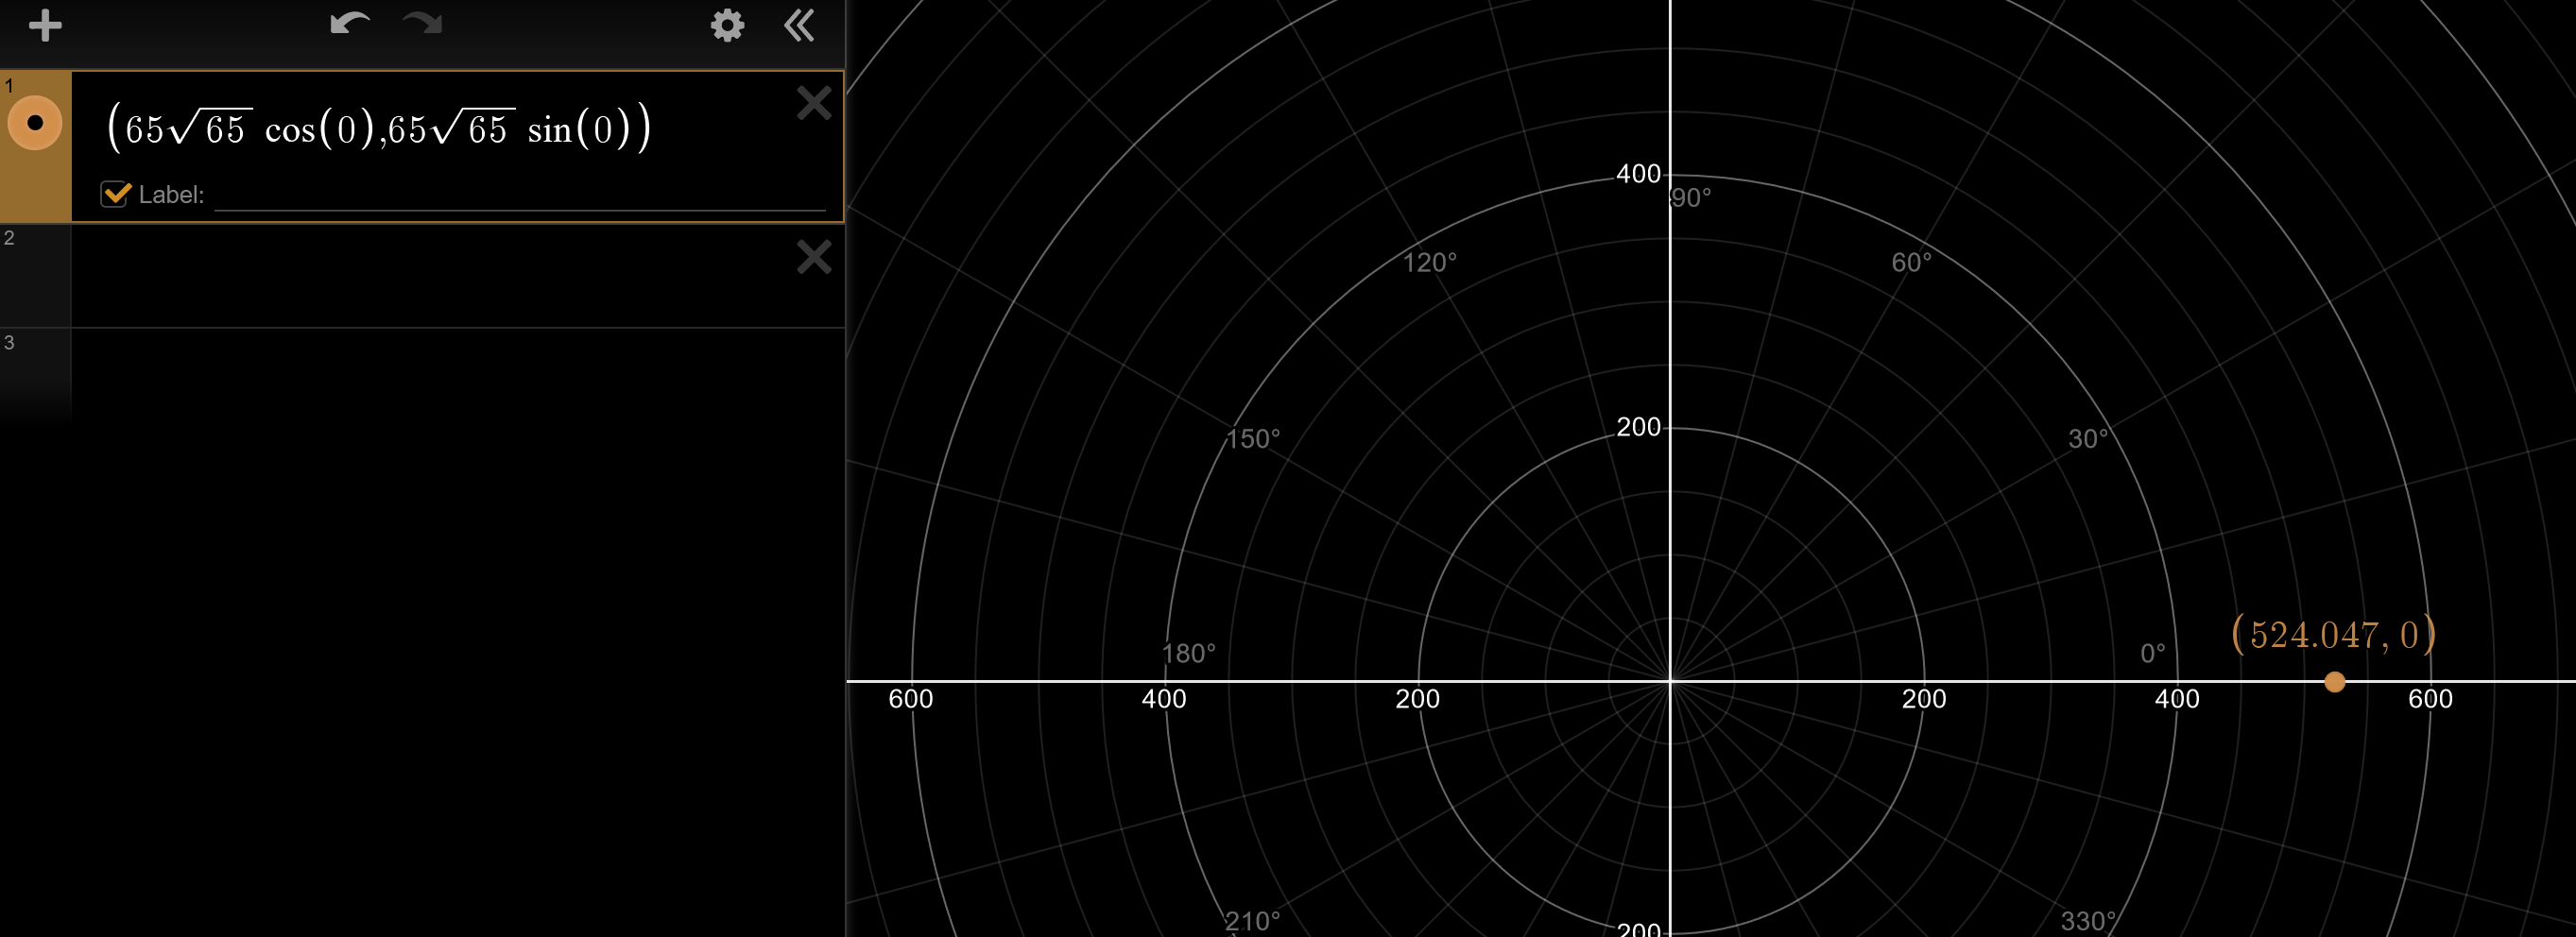
\includegraphics[width=\textwidth]{2}

$$(\sqrt{65}(\cos120\degree+i\sin120\degree))^-2 = \frac{1}{\sqrt{65}^2}(\cos-2\cdot120\degree+i\sin-2\cdot120\degree)= \frac{1}{65}(\cos120\degree + i\sin120\degree)$$

$$\frac{1}{65}(\cos120\degree + i\sin120\degree)=\frac{1}{65}(-\frac{1}{2}+\frac{\sqrt{3}}{2}i) = -\frac{1}{130}-\frac{\sqrt{3}}{130}i$$

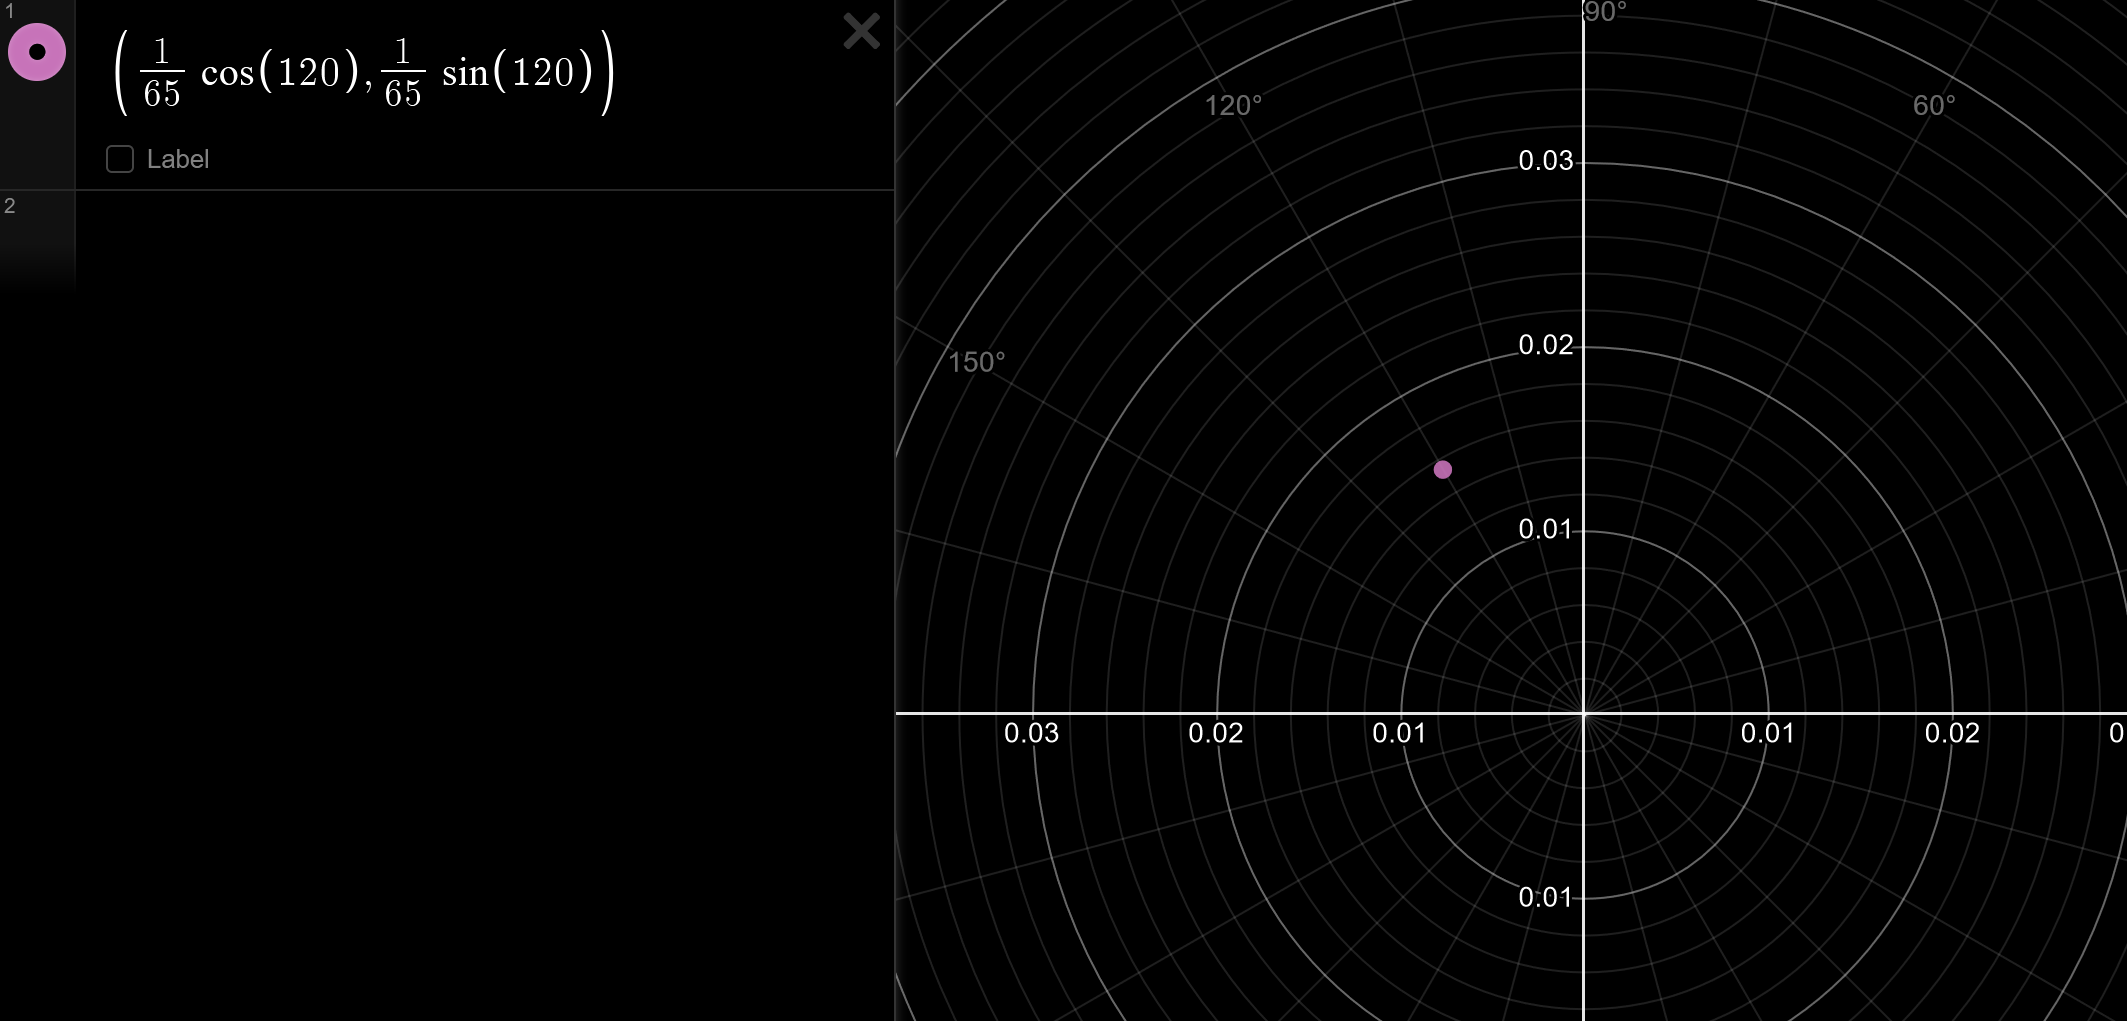
\includegraphics[width=\textwidth]{3}
\end{document}